\setcounter{chapter}{0}
\setcounter{secnumdepth}{-1}

\chapter{\label{sec:intro}Introduction}

The field of particle physics seeks to understand the nature of matter at a fundamental level. Physicists have always wished to know how mass and energy come about and how they interact with each other and the universe. Democritus' hypothesis of the atomic structure of matter, put forth over 2500 years ago, has prevailed as one of the most profound advancements in the natural sciences. Yet, only in the last two centuries have we made progress in identifying and categorizing the basic constituents that compose this universe.

\begin{figure}[b]
\begin{center}
    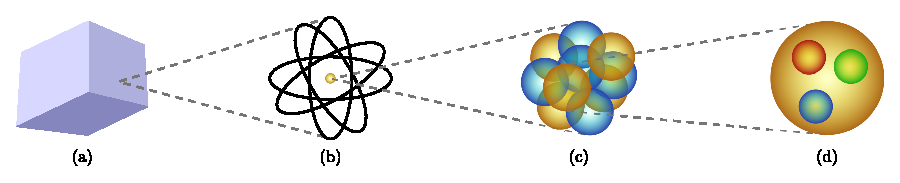
\includegraphics[width=0.9\columnwidth]{\figures/intro/constituents_of_matter.eps}
    \caption[History of Matter]{\label{fig:matter}A block of matter (a) is made of atoms (b) which consist of electrons orbiting a positively charged nucleus (c). The nucleus is comprised of protons and neutrons which are each made of three \emph{valence} quarks (d).}
\end{center}
\end{figure}

Great progress has been made in our understanding of matter starting with the discovery of the atom as an electrically positive nucleus surrounded by negatively charged electrons as proposed by Rutherford and Bohr\cite{rutherford1911} in 1911 and depicted in Fig.~\ref{fig:matter}(b). It was found by Chadwick\cite{chadwick1932} in 1932 that the nucleus consists of protons and neutrons, and in 1937, Stern et.\ al.\cite{PhysRev.52.535} found evidence that protons were not point-like as electrons seemed to be, but had some internal structure. During the ensuing couple decades, collider experiments revealed new particles that did not fit the proton-neutron-electron scheme of matter, and several new classes of subatomic particles including K-mesons and hyperons were identified.

In 1964, Gell-Mann organized many of these experimentally seen particles into what he called the \emph{eightfold way}. For the first time, subatomic particles were organized so that their properties and quite literally their very existence could be predicted. In fact, Gell-Mann's organizational model successfully predicted the existence\cite{barnes1964} of an unknown particle known today as the $\Omega^-$ baryon. From all the known resonances that were observed (more than 20 at the time) Gell-Mann found that he could describe their properties quite naturally by the existence of three constituents --- the up, down and strange \emph{quarks} which have half-integer spin and fractional electric charge. Over the past 50 years, three additional, heavier quarks have been added for a total of six which are categorized into three (and likely not more than three\cite{DeCamp1989,Blondel2002}) ``generations'' as shown in Table~\ref{tab:quarks}\footnote{In this work, we use units where the speed of light ($c$) and Planck's constant ($\hbar$) are equal to unity, making the units for mass, energy and momentum that of electron-volts (eV); the division by multiples of $c$ is implied.}.

\begin{table}
\begin{minipage}{\textwidth}
\begin{center}
\begin{singlespacing}

\caption[Quarks in the Standard Model]{\label{tab:quarks}The six \emph{flavors} of quarks which make up all hadronic matter in the Standard Model. All have spin $\frac{1}{2}$. The \emph{current-quark} mass is shown in MeV for each\cite{pdg}.}

\begin{tabular}{c|ccc}

\hline \hline

electric & \multicolumn{3}{c}{Generation} \\
charge & I & II & III \\


\hline

\multirow{2}{*}{$\frac{2}{3}$} & up ($u$) & charm ($c$) & top ($t$) \\
 & 3 & 1300 & 171k \\

\hline

\multirow{2}{*}{$-\frac{1}{3}$} & down ($d$) & strange ($s$) & bottom ($b$) \\
 & 5 & 105 & 4.2k \\

\hline \hline

\end{tabular}

\end{singlespacing}
\end{center}
\end{minipage}
\end{table}
\vspace{20pt} % tab:quarks

This theory, for which Gell-Mann won the Nobel Prize, formed the basis for what is known as the Standard Model of particle physics. The ideas behind this model retained the atomic structure of matter, and extended it to the interacting forces between particles. Protons and neutrons became part of a family of particles called \emph{hadrons}, while electrons became part of a family of particles called \emph{leptons}. The forces between these particles were then mediated by exchange of other particles called \emph{bosons}; the photon for example is the force carrier of the electromagnetic interaction.

Hadrons are complex particles making them difficult to understand. Unlike the simpler point-like leptons, they are composed of two or more quarks and/or anti-quarks. The quarks themselves carry a unique three dimensional charge called color. The color-charge for quarks can be one of three colors: red, blue or green. The color-charge for anti-quarks can be one of three colors: anti-red, anti-blue and anti-green.

Quarks and anti-quarks do not exist in isolation, but are found only in specific combinations. Experimental observation has shown these combination to be colorless. Three quarks in combination, whose colors are red, blue and green, are colorless. One quark and one anti-quark in combination with opposite colors, such as red and anti-red, is also colorless. The three-quark combination is called a \emph{baryon} and the quark-anti-quark combination is called a \emph{meson}.

This dissertation describes the work done to gain understanding of nucleon structure via measurement of the excitations of \emph{baryons}, the lowest lying states (lowest in terms of mass) which can be organized by SU(3) symmetry\cite{hassani2000}, using the three lightest quarks: \emph{up}, \emph{down} and \emph{strange}, as shown in Fig.~\ref{fig:baryons.eightfoldway}. Quantum chromodynamics, or \abbr{QCD}, is the leading theory to describe the strong force or the interactions between quarks which give rise to the nucleon structure. However, it is analytically insoluble and only recently have computing techniques with lattice \abbr{QCD} been able to produce reliable results.

\input{figures/tex/baryons_eightfoldway} % fig:baryons.eightfoldway

The modern formalism used to describe mass and the forces governing the interaction between masses is not the familiar $F=ma$ of Newton, but what is known as Lagrangian formulation. This is a way of encoding the equations of motion so that symmetries that correspond to conservation laws become easily accessible. The formulation consists of a single function, called the Lagrangian, which contains all the fundamental particle interactions. It is an abstraction from which the equivalent of $F=ma$ may be derived --- though generally this is not done directly. Furthermore, we currently lack the capability to do so analytically for the ``strong'' interactions between quarks. The Lagrangian of \abbr{QCD} ($\Lqcd$) which governs the interactions of quarks and their intermediary fields, gluons, is given as
\begin{equation}
    \Lqcd =
    \qbarfield_i
    \left( i \gamma^\mu \left( D_\mu \right)_{ij} - m \delta_{ij} \right)
    \qfield_j
    - \frac{1}{4}G^{a}_{\mu\nu}G^{\mu\nu}_{a},
    \label{eqn:qcd_lagrangian}
\end{equation}
where $\qfield_i$ is the quark field of flavor $i$, $G^{a}_{\mu\nu}$ is the gluon field strength tensor for color-charge $a$:
\begin{equation}
    G^{a}_{\mu\nu} =
    \partial_\mu G^{a}_{\nu}
    - \partial_\nu G^{a}_{\mu}
    - g f_{abc} G^{b}_{\mu} G^{c}_{\nu},
    \label{eqn:gluon_field_tensor}
\end{equation}
and $m$ is the mass of the quark. The term $\left( D_\mu \right)_{ij}$ consists of the self interaction for the quarks and the interaction between the quarks and the gluon fields:
\begin{equation}
    \left( D_\mu \right)_{ij}
    = \partial_\mu \delta_{ij} - g G^a_\mu \gamma^\mu T^a_{ij}.
    \label{eqn:gellmann_derivative}
\end{equation}
Inserting this into the Lagrangian yields
\begin{equation}
    \Lqcd =
    i \qbarfield_i \gamma^\mu \partial_\mu \qfield_i
    - \qbarfield_i m \qfield_i
    - g \qbarfield_i G^a_\mu \gamma^\mu T^a_{ij} \qfield_j
    - \frac{1}{4} G^a_{\mu\nu}G^{\mu\nu}_a,
    \label{eqn:qcd_lagrangian_expanded}
\end{equation}
where the first term is quark self interaction, the second term depends on the quark mass (a subtle issue that is discussed later), the third is the quark-gluon interaction, and the last term contains the gluon-gluon interaction. The $T^{a}_{ij}$ are the SU(3) generators which can be represented by the Gell-Mann matrices --- these are the SU(3) analog of the Pauli matrices. In the quark-gluon interaction term, $g$ is a constant and the same for all quarks. It may scale with the energy of the interaction, but is flavor independent. Therefore, this theory suggests all quark-gluon interactions are independent of quark flavor.

Notice, the mass term (second in Eq.~\ref{eqn:qcd_lagrangian_expanded}) is the only one that is dependent on the quark flavor. Therefore, as far as \abbr{QCD} is concerned, the quark-quark interaction should manifest itself with a simple relation between the masses of particles made of \abbr{QCD} quarks. A direct consequence of this is that the excitation spectra of baryons, three quark states whose binding energy is dominated by \abbr{QCD}, should be independent of the flavor of the constituent quarks. Moreover, the light baryon resonances, those made from up and down quarks only, will be governed by the same interactions as the doubly-strange baryons (i.e.\ those with two strange quarks and one up or down quark). The result is that the spectra of these two will have nearly identical shapes. Each light octet (N$^*$) and decuplet ($\Delta^*$) state will have a corresponding octet or decuplet $\Xi^*$ state. This will also hold for singly-strange baryons as discussed in the following sections. The phrase ``nearly identical'' was used because the doubly-strange \emph{cascade} states have two identical strange quarks and therefore their spectrum contains no singlets, so there are no $\Xi^*$ analogs to the singlet $\Lambda^*$ states for example.

A perfect one-to-one correlation should not be expected. There will be electro-weak corrections due to the charge of the quarks via quantum electrodynamics (\abbr{QED}). Furthermore, there are spin-spin and spin-orbit energies that can contribute a shift in the mass differences when a $d$ quark is replaced by an $s$ quark. Once all these effects are taken into account, mismatching states in the spectra can be interpreted as some new physics not included in $\Lqcd$ of Eq.~\ref{eqn:qcd_lagrangian}.

The masses shown in Table~\ref{tab:quarks} are what is known as the \emph{bare} or \emph{current}-quark masses. These are the best estimates of what the masses would be for free quarks --- that is, outside the influence of an external \abbr{QCD} potential. These values are the quark masses that would be inserted into the \abbr{QCD} Lagrangian provided it was solvable analytically, but there are certain problems with these estimates.

Discussions on masses of particles that can not be measured directly become philosophic in nature quickly. However, a brief investigation into this subject is necessary at this point. In a na\"ive model, one could say that there are three quarks ($uud$) in a proton of mass 938~MeV and therefore they are approximately one third its mass which comes to 313~MeV. This is obviously much higher than the values given in Table~\ref{tab:quarks}. There are other particles we could look at besides the proton. For example, the pion is composed of two light quarks (up and down) and has a mass of 140~MeV which brings the mass of the up and down quarks to around 70~MeV. Still higher than quoted, but much closer.

So what might be going on here? The current-quark theory suggests these light quarks (a few MeV for the \emph{up} and \emph{down}) are surrounded by a ``bubbling sea'' of gluons and short-lived quark/anti-quark pairs. The interactions of these particles coming in and out of existence constantly on very short time scales effectively adds the mass that is ``missing'' to the hadronic particles. Even with all the calculations made and data collected on this subject\cite{pdg}, there is a lot of controversy on these vital ingredients to the Standard Model and \abbr{QCD} and more data is needed.

The cascade states provide an accessible way to study the up/down quark mass difference. Since the two strange quarks are much more massive than the other light (up or down) quark, interchanging the light quark with another is a relatively small change on the whole system. Therefore, the effect of this switch is isolated.

This dissertation presents an analysis of the lowest lying doubly-strange baryons and the comparison to the known light and singly-strange baryon spectra. The goal is to show the extent to which the strong force is flavor independent. If the three spectra have a one-to-one correspondence where the differences can be fully explained (by mass differences, \abbr{QED}, etc.) then the \abbr{QCD} Lagrangian as written in Eq.~\ref{eqn:qcd_lagrangian} will have deeper experimental support. If a discrepancy can be identified, this will be an indication that a modification of the \abbr{QCD} Lagrangian would be required.

\setcounter{secnumdepth}{2}

\input{intro/cascades}
\input{intro/predicted}
\input{intro/evidence}
\section{\label{sec:results.exotics}Search for \emph{Iso-exotic} States}

patented exotic such as the Sigma-- Sigma++ Xi-- and Xi+ at ``best estimate'' masses and widths.

\begin{table}
\begin{minipage}{\textwidth}
\begin{center}
\begin{singlespacing}
\caption[Exotic States Upper Limits]{\label{tab:exotic.ulimits}Upper limit cross sections for the exotic states.}
\begin{tabular}{lcccc}
\hline \hline
state & $F$ & $<N$ & $A$ (\%) & $<\sigma$ (nb) \\
\hline
$\Xi^+$       &  & \\
$\Xi^{--}$    &  & \\
$\Sigma^{++}$ &  &  \\
$\Sigma^{--}$ &  &  \\
\hline \hline
\end{tabular}
\end{singlespacing}
\end{center}
\end{minipage}
\end{table}


\begin{figure}[bh]\begin{center}
    \includegraphics[width=0.8\figwidth]{\figures/analysis/mmkpkppip.eps}
    \caption[MM(K$^{+}$K$^{+}\piup^+$)]{\label{fig:mmkpkppip}Missing mass off K$^{+}$K$^{+}\piup^+$ in the reaction $\gammaup \p \rightarrow \Kp \Kp \piup^+ X^{--}$ with cuts as described in Tables~\ref{tab:vtime.cuts} and \ref{tab:kpkp.cuts}.}
\end{center}\end{figure}

\clearpage

